% --
%
% Configuração do Documento
%
% --
\documentclass[10pt,brazil]{beamer}
\uselanguage{Portuguese}
\languagepath{Portuguese}
\usepackage[utf8]{inputenc}


% ---
% Pacotes adicionais
% ---
\usepackage[light,math]{kurier}         %Altera Fonte Utilizada no arquivo
\usepackage{amsmath,amsfonts,amsthm,amssymb,mathrsfs}
\allowdisplaybreaks[1]
\usepackage{microtype}
\usepackage{listings}
\usepackage{mathtools}
\usepackage{csquotes}
\usepackage{tikz}
\usepackage{animate}
\usetikzlibrary{matrix}
\usetikzlibrary{patterns}
\usepackage{faktor}
\usepackage[Sonny]{fncychap}
\usepackage{hyperref}
\usepackage{tikz}
\graphicspath{{images/}}
\usepackage[light,math]{kurier}
\usetheme{Madrid}
\useinnertheme{rectangles}


\renewcommand{\raggedright}{\leftskip=0pt \rightskip=0pt plus 0cm} %texto justificado

\usepackage[%
    alf,
    abnt-emphasize=bf,
    bibjustif,
    recuo=0cm,
    abnt-doi=expand,            % Expande um endereço iniciado com doi: para http://dx.doi.org/
    abnt-url-package=url,       % Utiliza o pacote url
    abnt-refinfo=yes,           % Utiliza o estilo bibliográfico abnt-refinfo
    abnt-etal-cite=3,
    abnt-etal-list=3,
    abnt-thesis-year=final
]{abntex2cite}   

\setbeamertemplate{theorems}[numbered] % to number
\setbeamercovered{transparent}

\theoremstyle{definition}
\newtheorem{dfn}{Definição}
\newtheorem{obs}{Observação}
\newtheorem*{proofthm}{Demonstração do Teorema}
\newtheorem*{proofprop}{Demonstração da Proposição}
\newtheorem{ex}{Exemplo}
\newtheorem{prop}{Propriedade}
\newtheorem{proposition}{Proposição}


\newcommand{\der}{\text{d}}					%Comando para fazer o d da derivada fora do ambienta matemático
\newcommand{\mb}[2]{\mathbb{#1}^{#2}}		%Comando para usar \mathbb de maneira  mais eficiente
\newcommand{\mca}[2]{\mathcal{#1}_{#2}}
\newcommand{\mul}[2]{\mu_{#1}\left(#2\right)}			%Comando para escrever a multiplicidade de modo mais eficiente
\newcommand{\mc}[2]{\mathcal{I}_{#1}\left(#2\right)}   %Comando para escrever o IPH de maneira  mais eficiente

% --
% Define Cores Personalizadas 
% --
\definecolor{ver}{RGB}{124,26,29}
\definecolor{yel}{RGB}{158,134,35}
\definecolor{ros}{RGB}{255,51,102}
\definecolor{ver1}{RGB}{169,88,99}
\definecolor{ver2}{RGB}{156,63,75}
\definecolor{ver3}{RGB}{145,43,56}
\definecolor{azul}{RGB}{18,35,97}

% --
% Customiza o título 
% --
\setbeamercolor{title}{fg=azul, bg=white!95!black}

% --
% Remove os controles de navegação 
% --
\setbeamertemplate{navigation symbols}{}

% --
% Customiza o background
% --
\setbeamertemplate{background}{
	\begin{tikzpicture}[remember picture,overlay]
	% --- LinhaInferior
	\draw[line width=0.4mm,azul] ([shift={(2.5cm,0.4cm)}]current page.south west) -- ([shift={(-0.38cm,0.4cm)}]current page.south east);
	\draw[line width=0.4mm,azul] ([shift={(-0.3cm,0.4cm)}]current page.south east) -- ([shift={(-0.26cm,0.4cm)}]current page.south east);
	\draw[line width=0.4mm,azul] ([shift={(2.75cm,0.3cm)}]current page.south west) -- ([shift={(-0.38cm,0.3cm)}]current page.south east);
	\draw[line width=0.4mm,azul] ([shift={(-0.3cm,0.3cm)}]current page.south east) -- ([shift={(-0.26cm,0.3cm)}]current page.south east);
	\draw[line width=0.4mm,azul] ([shift={(3cm,0.2cm)}]current page.south west) -- ([shift={(-0.38cm,0.2cm)}]current page.south east);
	\draw[line width=0.4mm,ver1] ([shift={(-0.3cm,0.2cm)}]current page.south east) -- ([shift={(-0.26cm,0.2cm)}]current page.south east);
	
	% --- Logo 
	\node[xshift=-1.5cm,yshift=-0.8cm] at (current page.north east) {
\includegraphics[scale=0.15]{logo_ufmg.jpg}};
	
	\end{tikzpicture}
}

% --
% Customiza o título do frame 
% --
\setbeamercolor{frametitle}{fg=azul, bg=white} 
\makeatletter
\setbeamertemplate{frametitle}
{
	\ifbeamercolorempty[bg]{frametitle}{}{\nointerlineskip}%
	\@tempdima=\textwidth%
	\advance\@tempdima by\beamer@leftmargin%
	\advance\@tempdima by\beamer@rightmargin%
	\pgfsetfillopacity{.1}       %<------ fix filling opacity
	\begin{beamercolorbox}[sep=0.3cm,left,wd=\the\@tempdima]{frametitle}
		\usebeamerfont{frametitle}%
		\vbox{}\vskip1ex \hskip6ex%
		\if@tempswa\else\csname beamer@fteleft\endcsname\fi%
		\strut\pgfsetfillopacity{1}\insertframetitle\strut\par%  <---- text opacity
		{%
			\ifx\insertframesubtitle\@empty%
			\else%
			{\usebeamerfont{framesubtitle}\usebeamercolor[fg]{framesubtitle}\insertframesubtitle\strut\par}%
			\fi
		}%
		\vskip-1ex%
		\if@tempswa\else\vskip-.3cm\fi% set inside beamercolorbox... evil here...
	\end{beamercolorbox}%
}
\makeatother


% --
% Customimza o ambiente de Teorema 
% --
\setbeamercolor{block title}{use=structure, fg=white, bg=azul}
\setbeamercolor{block body}{use=structure, fg=black, bg=white!96!black}
\setbeamertemplate{block begin}[default]
\setbeamertemplate{block end}[default]



% --
% Customiza o footline 
% --
\defbeamertemplate{footline}{centered page number}
{%
  \hspace*{\fill}%
  \usebeamercolor[fg]{page number in head/foot}%
  \usebeamerfont{page number in head/foot}%
  \insertpagenumber\,/\,\insertpresentationendpage%
  \hspace*{\fill}%
  \hspace*{\fill}%
  \hspace*{\fill}%
  \hspace*{\fill}%
  \hspace*{\fill}%
  \hspace*{\fill}%
  \hspace*{\fill}%
  \hspace*{\fill}%
  \hspace*{\fill}
  \hspace*{\fill}%
  \hspace*{\fill}%
  \hspace*{\fill}%
  \hspace*{\fill}\vskip6pt%
}
\setbeamertemplate{footline}[centered page number]

% --
% Customiza o headline 
% --
\setbeamertemplate{headline}
{
	\leavevmode%
	\hbox{%
		\begin{beamercolorbox}[wd=\paperwidth,dp=3.5ex]{ver}%
			\raggedright
			\hspace*{2em}%
		\end{beamercolorbox}%
	}%
}


% --
% Customiza o estilo dos ambientes Itemize e Enumerate 
% --
\setbeamertemplate{enumerate item}{\color{azul}\insertenumlabel)}
\setbeamertemplate{enumerate subitem}{\color{azul}\insertenumlabel.\insertsubenumlabel)}
\setbeamertemplate{enumerate subsubitem}{\color{azul}\insertenumlabel.\insertsubenumlabel.\insertsubsubenumlabel)}
\setbeamertemplate{enumerate mini template}{\insertenumlabel}

\setbeamertemplate{itemize item}{\scriptsize\raise1.25pt\hbox{\color{azul}\donotcoloroutermaths$\bullet$}}
\setbeamertemplate{itemize subitem}{\tiny\raise1.5pt\hbox{\color{azul}\donotcoloroutermaths$\blacksquare$}}
\setbeamertemplate{itemize subsubitem}{\tiny\raise1.5pt\hbox{\color{azul}\donotcoloroutermaths$\blacktriangleright$}}

% -- 
% Customiza o estilo do Table of Contents 
% --
\setbeamertemplate{section in toc}[square]

\setbeamerfont{section number projected}{size=\large}
\setbeamercolor{section number projected}{bg=white!95!black, fg=azul}

\setbeamertemplate{subsection in toc}{%
	\leavevmode\leftskip=5.65ex%
	\llap{\raisebox{0.2ex}{\textcolor{azul}{$\bullet$}}\kern1ex}%
	\inserttocsubsection\par%
}

% -- 
%Customiza as margens dos frames 
% -- 
\setbeamersize{text margin left=1cm,text margin right=1cm}

% -- 
% Apresentação
% -- 
\begin{document}
\mode<presentation>

% -- 
% Info
% -- 
\title[]{ANÁLISE DE DADOS UTILIZANDO \emph{CLUSTER} DE BAIXO CUSTO}
\subtitle{Tendências de consumo da
azitromicina no Brasil antes e durante a
pandemia da COVID-19}

\institute[UFMG]{Universidade Federal de Minas Gerais}

\author[Felipe Rocha]{Felipe Fonseca Rocha \\
  \vspace{0.25cm}
  Orientador: Ítalo Fernando Scotá Cunha}
\date{09 de Fevereiro de 2022}

% --
% Inclui o sumário antes de cada seção
% --
\AtBeginSubsection{%
  \begin{frame}
    \tableofcontents[currentsection=show,sectionstyle=show/shaded,subsectionstyle=show/shaded/hide]
  \end{frame}
}
% -- 
% Cria slide com título
% -- 
\frame{\maketitle}

% -- 
% Cria slide com sumário
% -- 

\begin{frame}{Sumário}
  \tableofcontents[hideallsubsections]
\end{frame}

% 	\begin{figure}
% 		\centering
% 		\includegraphics[scale=0.45]{objetivo.jpg}
% 	\end{figure}

% --
%
% Conteúdo 
%
% --

% -- 
% Introdução
% -- 
\section{Contexto e Motivação}
% -- 
% Motivação [allowframebreaks]
% -- 
\subsection*{Contexto de Dados}
\begin{frame}{Contexto de Dados - produção e uso}
  \begin{columns}
    \begin{column}{0.5\textwidth}
      \begin{itemize}
        \item[] A todo momento nós geramos milhões de dados que são coletados por diferentes meios
        \item[]
        \item[] Existem várias ferramentas disponíveis para transformá-los em informações e embasar decisões
      \end{itemize}
      %\cite{galvao_desafios_2019,mehta_concurrence_2018,brasildisponibilidade2016}
    \end{column}
    \begin{column}{0.5\textwidth}
      \begin{center}
        
\includegraphics[width=1\textwidth]{sis.png}
      \end{center}
    \end{column}
  \end{columns}
\end{frame}  
  \begin{frame}{Contexto de Dados - Área da Saúde}
    \begin{columns}
    \begin{column}{0.5\textwidth}
    \begin{center}
      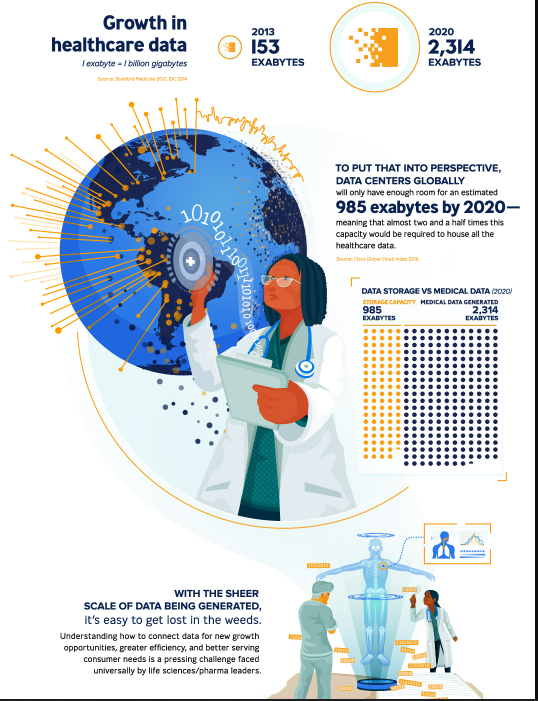
\includegraphics[width=.9\textwidth,height=.75\textheight]{growthhealth.png}
      \end{center}
    \end{column}
    \begin{column}{0.5\textwidth}
      \begin{itemize}
        \item[] Isso também acontece na área da saúde
        \item[]
        \item[] Porém o uso de ferramentas de \emph{big data} em saúde ainda é pouco significativo
        \item[]
        \item[] Boa parte dessas ferramentas implica processamento distribuído
      \end{itemize}
    \end{column}
  \end{columns}
\end{frame}
\begin{frame}{Contexto de Dados - Desafios}
  \begin{columns}%\begin{center}
      \begin{column}{0.5\textwidth}
  \begin{itemize}
    \item[] Potencial de melhora do sistema de saúde através de análise de dados
    \item[]
    \item[] Integrar times com trabalho interdisciplinar
    \item[]
    \item[] Uso de ferramentas e recursos já disponíveis de maneira correta
    %item[] Plataformas de isolamento entre sistemas
  \end{itemize}
    \end{column}
    \begin{column}{0.5\textwidth}
      \begin{center}
        
\includegraphics[width=1\textwidth]{interdisciplinar.png}
      \end{center}
      \end{column}
   %\item Necessário propor e validar estratégias que sejam viáveis e facilitem o processamento de análise de grande volume de dados produzido na área
  \end{columns}
 %\end{center}
 %\framebreak
 % \begin{itemize}
 %   \item No Brasil, dados do Sistema de Informação em Sáude (SIS) são disponibilizados desde 2016
 %   \item \textbf{Faltam recursos} e estratégias viáveis para essa elaboração.
 % \end{itemize}
\end{frame}


\section{Justificativa}

% -- 
% Justificava
% -- 
\subsection{Justificativa Social}

\begin{frame}{Apoio a melhores decisões}

      \begin{itemize}
            \item Tomada de decisão em saúde
            \item Escala: $152$ \textbf{milhões} dependem exclusivamente do SUS
            \item Restrição: Gasto de $R\$3.83$ por pessoa por dia
            \item Transformar dados em informação
            \item \textbf{Assertividade}
      \begin{itemize}
          \item Ações em saúde
          \item políticas publicas
      \end{itemize}
      \end{itemize}
 
\end{frame}

\subsection{Justificativa Econômica}

\begin{frame}{Restrições de orçamento a ciência}
  \begin{columns}
    \begin{column}{0.5\textwidth}
              \begin{itemize}
                \item Diminuição de verbas para ciência e tecnologia -$2,32\%$
      \end{itemize}
    \end{column}
    \begin{column}{0.5\textwidth}  %%<--- here
      \begin{center}
        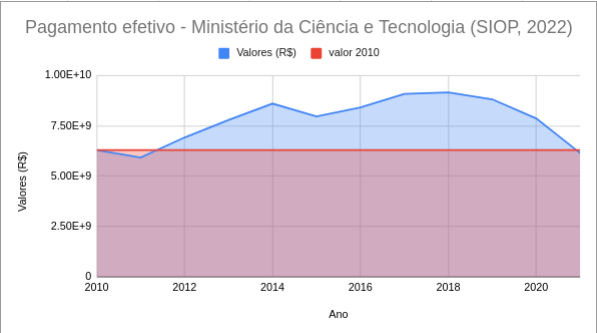
\includegraphics[width=1\textwidth]{orcamento.png}
        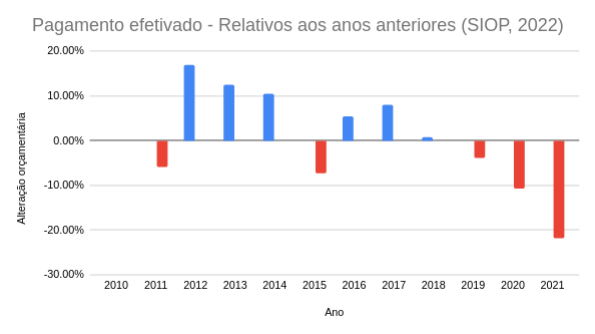
\includegraphics[width=1\textwidth]{variacaoorcamentaria.png}
      \end{center}
    \end{column}
  \end{columns}
\end{frame}

\begin{frame}{Alterações de cenário econômico}
  \begin{columns}
    \begin{column}{0.5\textwidth}
      \begin{itemize}
            \item Aumento do dólar em mais de $327\%$ diminuindo o poder de compra
            \item Aumento do custo de hardware e máquinas
      \end{itemize}
    \end{column}
    \begin{column}{0.5\textwidth}  %%<--- here
      \begin{center}
        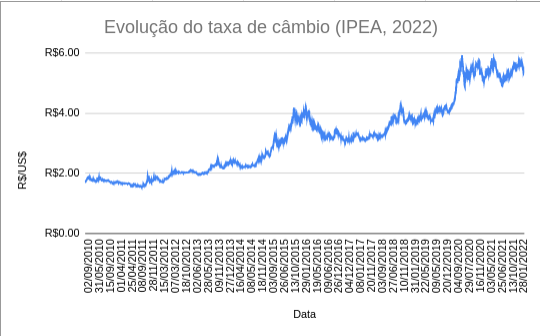
\includegraphics[width=1\textwidth]{variacaodolar.png}        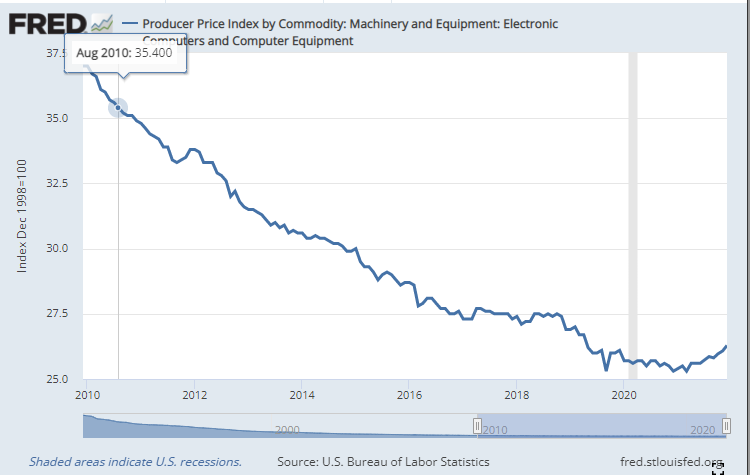
\includegraphics[width=1\textwidth]{hardwarecost.png}
      \end{center}
    \end{column}
  \end{columns}
\end{frame}

\subsection{Justificativa Técnica}

\begin{frame}{Viabilização de alternativas}
  \begin{columns}
    \begin{column}{0.5\textwidth}
      \begin{itemize}
            \item Necessário ser interdisciplinar
            \item Avaliar alternativas de processamento de dados 
            \item Amenizar questões orçamentá\-rias
            \item Melhorar uso dos recursos já exis\-tentes (e.g. inventário de universidades)
      \end{itemize}
  \end{column}
    \begin{column}{0.5\textwidth}  %%<--- here
      \begin{center}
        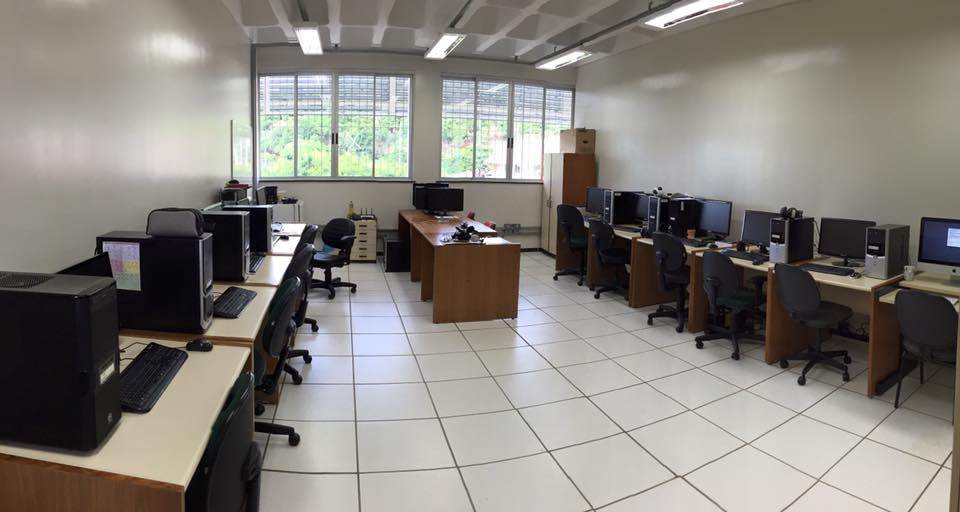
\includegraphics[width=1\textwidth]{lab.jpg}        
        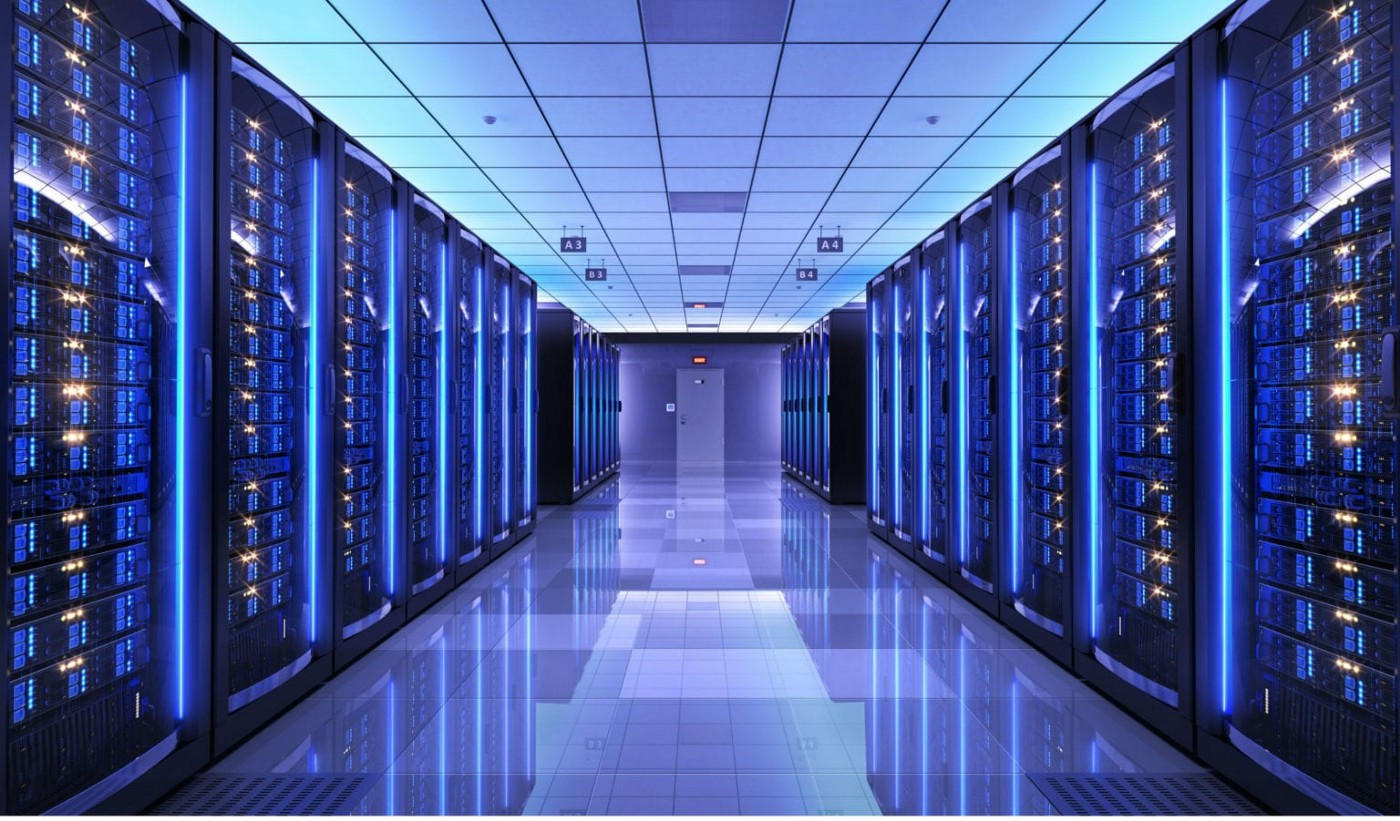
\includegraphics[width=1\textwidth]{hpc.jpeg}        
      \end{center}
    \end{column}
  \end{columns}
\end{frame}


% -- 
% Objetivos
% -- 
\section{Objetivo}
\subsection*{Objetivos Gerais}
%[allowframebreaks]
\begin{frame}{Objetivo}
  \begin{itemize}
    \item[] \textbf{Objetivos Geral:}
    \item[]
      \begin{itemize}
        \item[] Avaliar a viabilidade de orquestração de recursos em \emph{cluster} de baixo custo em ambientes containerizados, para o processamento e a análise dos dados.
      \end{itemize}
    \item[] \textbf{Objetivos Específicos:}
      \begin{itemize}
        \item Realizar a orquestração de recursos em \emph{cluster} de baixo custo;
        \item Avaliar tempo de provisionamento, tempo de execução e disponibilidade do cluster;
        \item Validar o uso de um \emph{cluster} de utilização compartilhada para processamento de dados distribuídos;
        \item Propor um método de análise em \emph{cluster} Kubernetes com uso de computadores desktops;
        \item Disponibilzar um cluster pronto para uso para UFMG, bem como ferramentas de auxilio no provisionamento;
      \end{itemize}
  \end{itemize}
\end{frame}


% -- F
% Revisão de Literatura
% -- 
\section{Revisão de literatura}

% -- 
%  Análise de dados
% -- 
% \subsection{Análise de dados}

% \begin{frame}{Análise de dados}
%   \begin{itemize}
%     \item Descisões em saúde costumam ser complexas - precisam de suporte científico (dados) e avaliação de Contexto
%     \item Com o crescimento dos 3V's de dados (Big Data), na área da saúde, processar e analisar esses dados tornou-se fundamental para tomada de descisões adequadas
%     \item Desafios:
%       \begin{itemize}
%         \item complexidade dos dados obtidos
%         \item ausência de validação de sistemas, métodos e ferramentas para o tratamento de dados na área
%         \item custos de novos equipamentos capazes de analisar tal volume
%       \end{itemize}
%     \item Há grande oportunidade para a proposição de estratégias de processamento e análise de dados nesse setor
%   \end{itemize}
% \end{frame}

% -- 
%  Alternativas open source
% -- 
\subsection{Alternativas \emph{open source}}

\begin{frame}{Alternativas \emph{open source}}
  \begin{itemize}
    \item Considerando
          \begin{itemize}
            \item O escopo deste trabalho
            \item Limitações de hardware
            \item As estratégias para processamento
            \item Ferramentas de análise de dados disponíveis no mercado
          \end{itemize}
    \item [] As soluções encontradas no mercado foram agrupadas em dois grupos:
          \begin{itemize}
            \item Soluções de Computação em nuvem privada:
                  \begin{itemize}
                    \item Se estendem para além do proposito desse trabalho
                    \item Requisitos de hardware elevados
                    \item Complexidade de configuração devido a sua abrangência
                  \end{itemize}
          \end{itemize}
  \end{itemize}
\end{frame}


\begin{frame}{Alternativas \emph{open source}}
  \begin{columns}
    \begin{column}{0.5\textwidth}
      \begin{itemize}
        \item Soluções de Orquestração de Containers:
              \begin{itemize}
                \item Kubernetes\textregistered
                \item Apache Mesos\textregistered
                \item Hashicorp Nomad\textregistered\*
                \item Docker Swarm\textregistered
              \end{itemize}
      \end{itemize}
    \end{column}
    \begin{column}{0.5\textwidth}  %%<--- here
      \begin{center}
        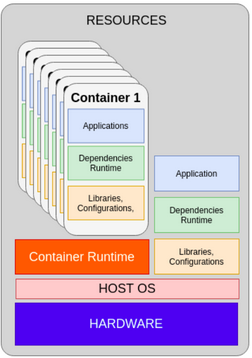
\includegraphics[width=1\textwidth]{containers.png}
        % 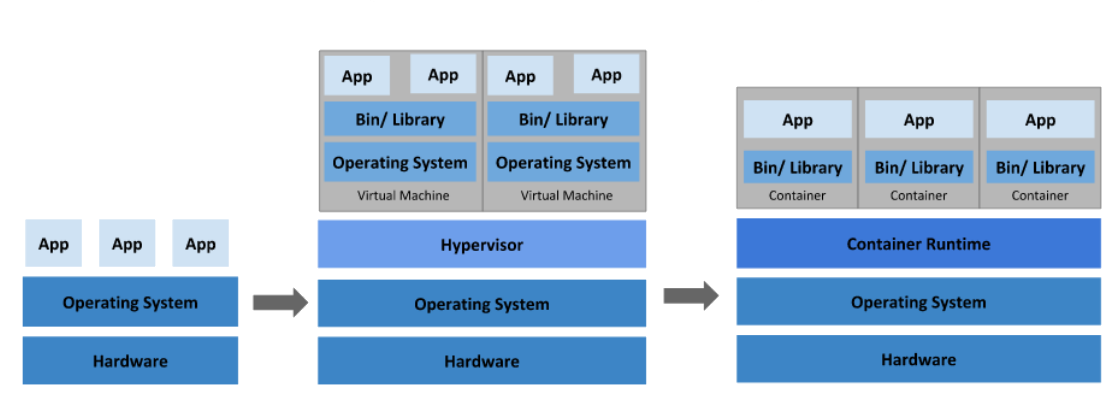
\includegraphics[width=1\textwidth]{vmsContainer.png}
      \end{center}
    \end{column}
  \end{columns}
\end{frame}

% -- 
% \emph{Cluster}orquestrador de container
% -- 
\subsection{Cluster orquestrador de container}

\begin{frame}{Cluster orquestrador de container}
  \begin{columns}
    \begin{column}{0.5\textwidth}
      \begin{itemize}
        \item Kubernetes\textregistered:
          \begin{itemize}
            \item Origem de 15 anos de trabalho da Google (Borg) %\cite{verma_large-scale_2015}
            \item Estrutura de objetos componentizados %\cite{kubernetes2022}
              \begin{itemize}
                \item Kube-apiserver
                \item Kube-scheduler
                \item Kube-controller-manager
                \item Kubelet
                \item Kube-proxy
                \item Pod
              \end{itemize}
          \end{itemize}
      \end{itemize}
    \end{column}
    \begin{column}{0.5\textwidth}  %%<--- here
      \begin{center}
        \begin{overprint}
          \onslide<1>
\includegraphics[width=1\textwidth]{k8s-1.png}
          \onslide<2>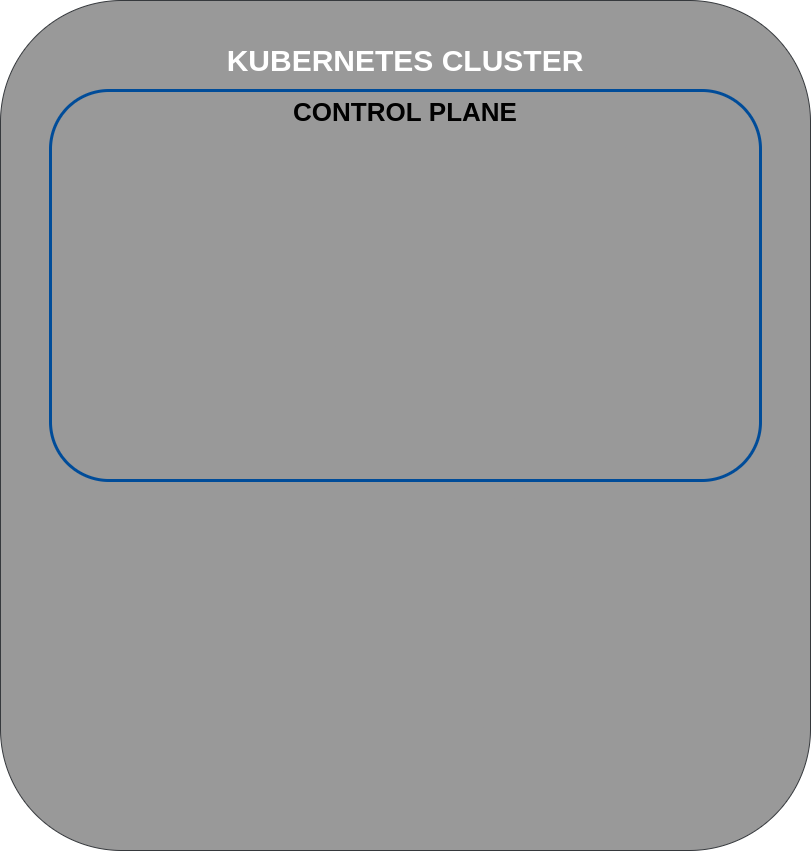
\includegraphics[width=1\textwidth]{k8s-2.png}
          \onslide<3>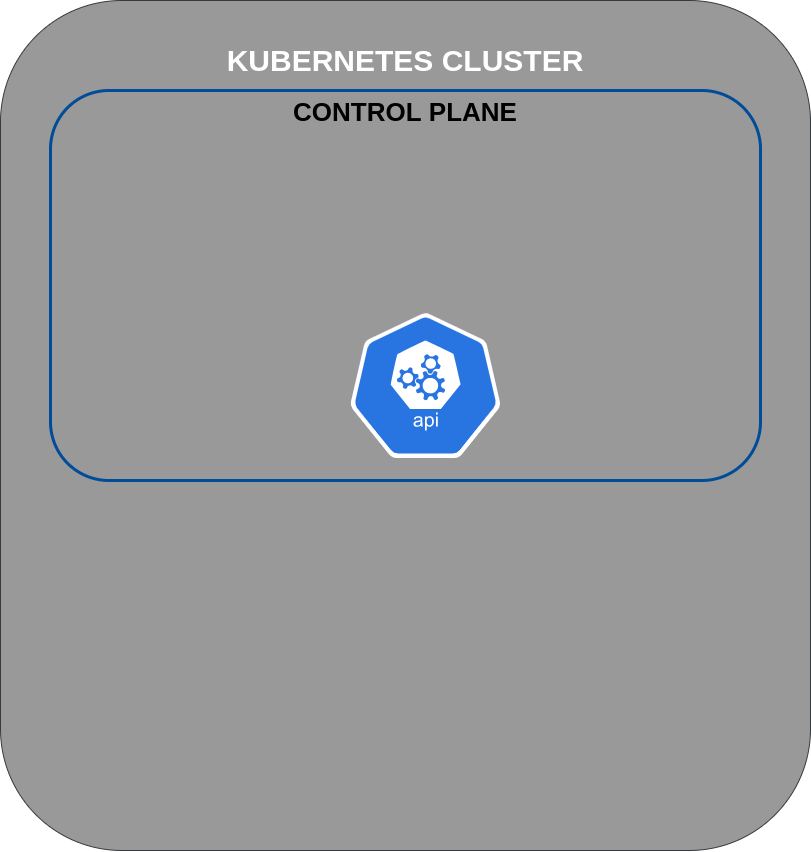
\includegraphics[width=1\textwidth]{k8s-3.png}
          \onslide<4>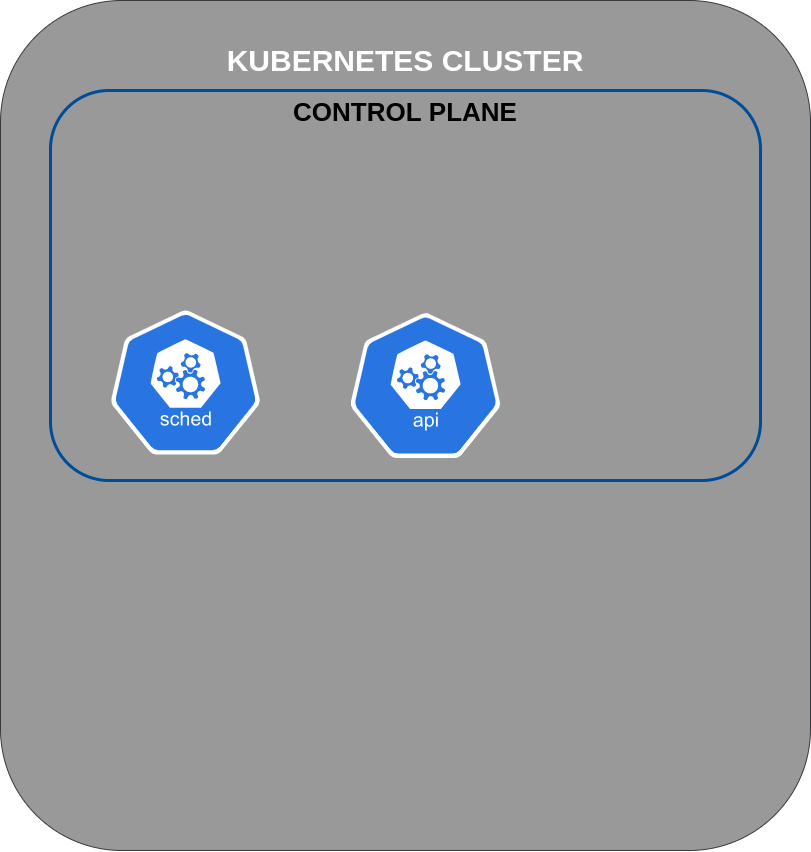
\includegraphics[width=1\textwidth]{k8s-4.png}
          \onslide<5>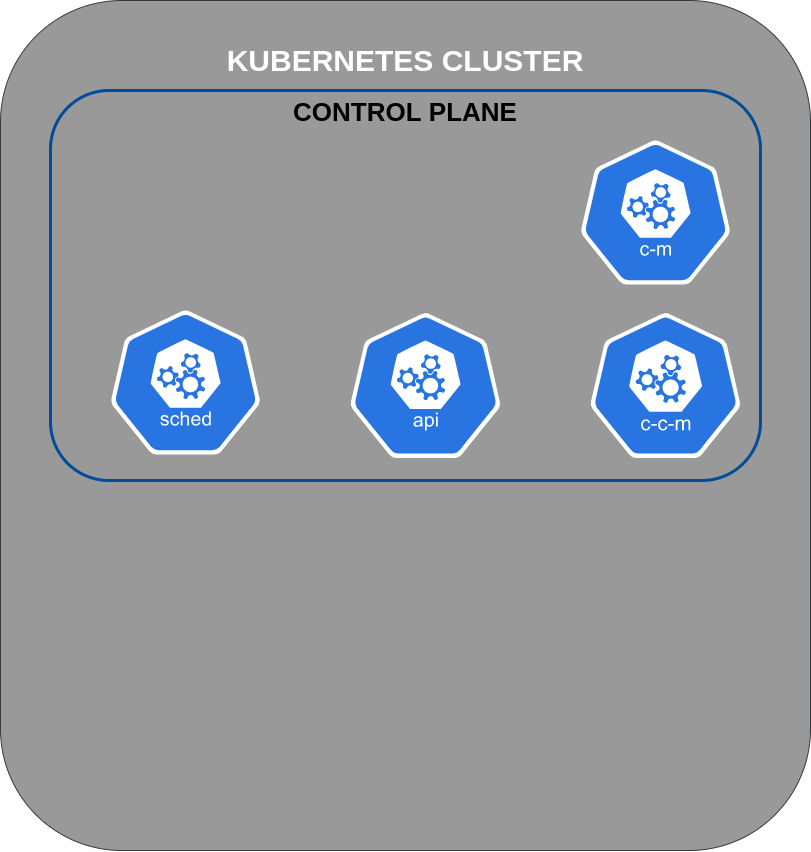
\includegraphics[width=1\textwidth]{k8s-5.png}
          \onslide<6>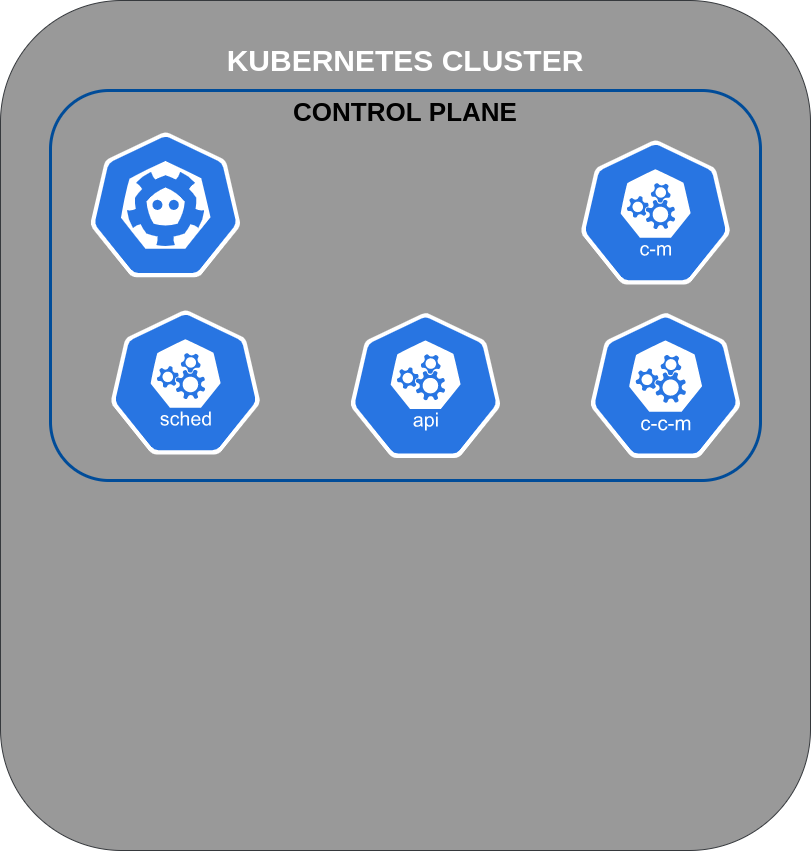
\includegraphics[width=1\textwidth]{k8s-6.png}
          \onslide<7>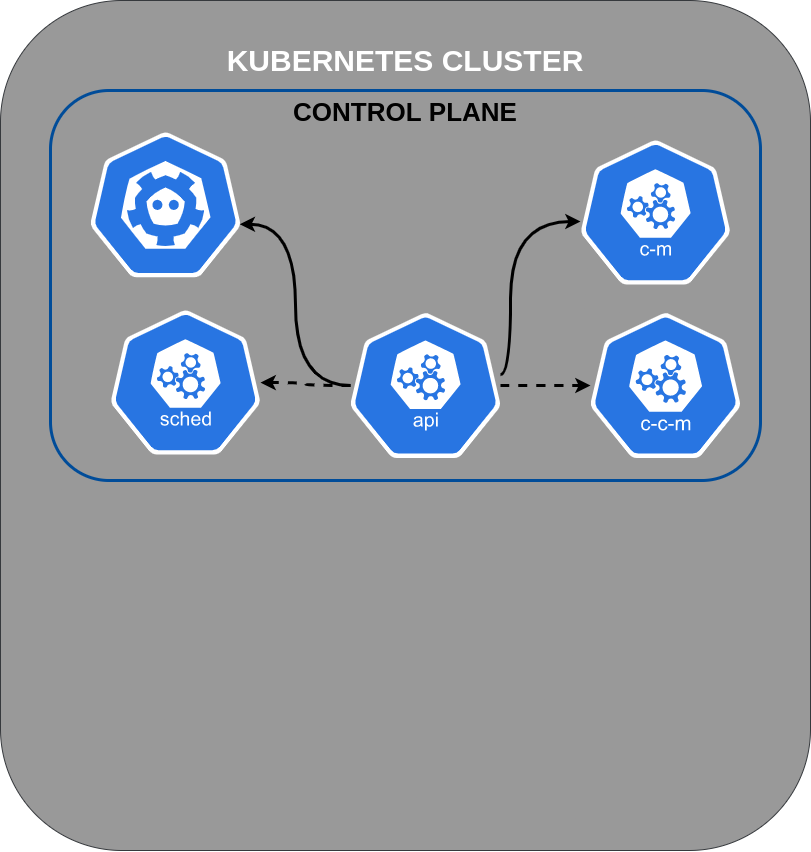
\includegraphics[width=1\textwidth]{k8s-7.png}
          \onslide<8>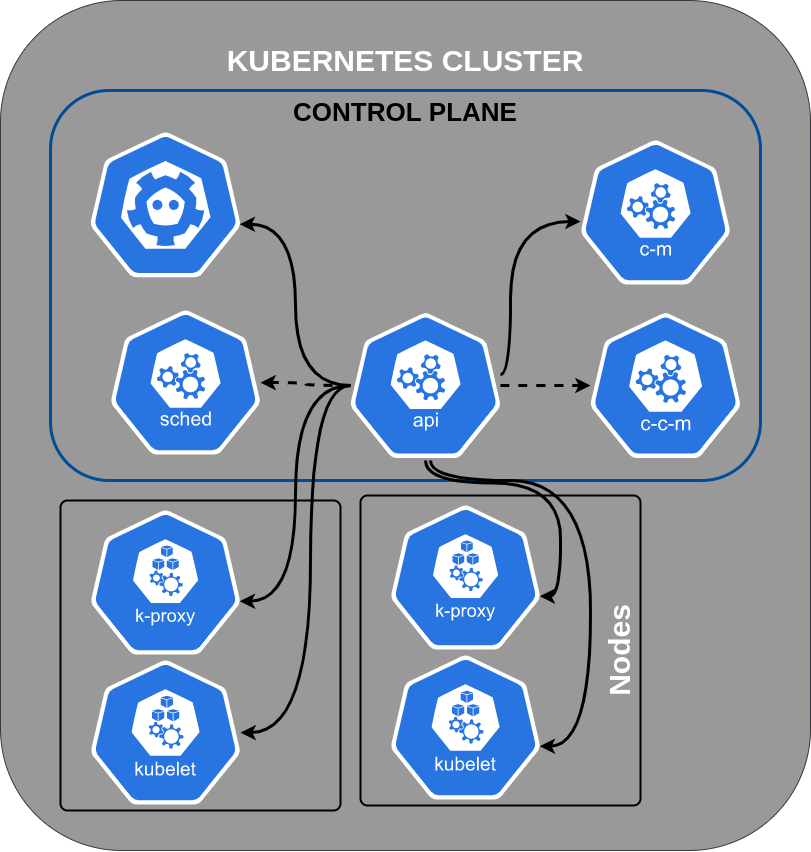
\includegraphics[width=1\textwidth]{k8s-8.png}
          \onslide<9->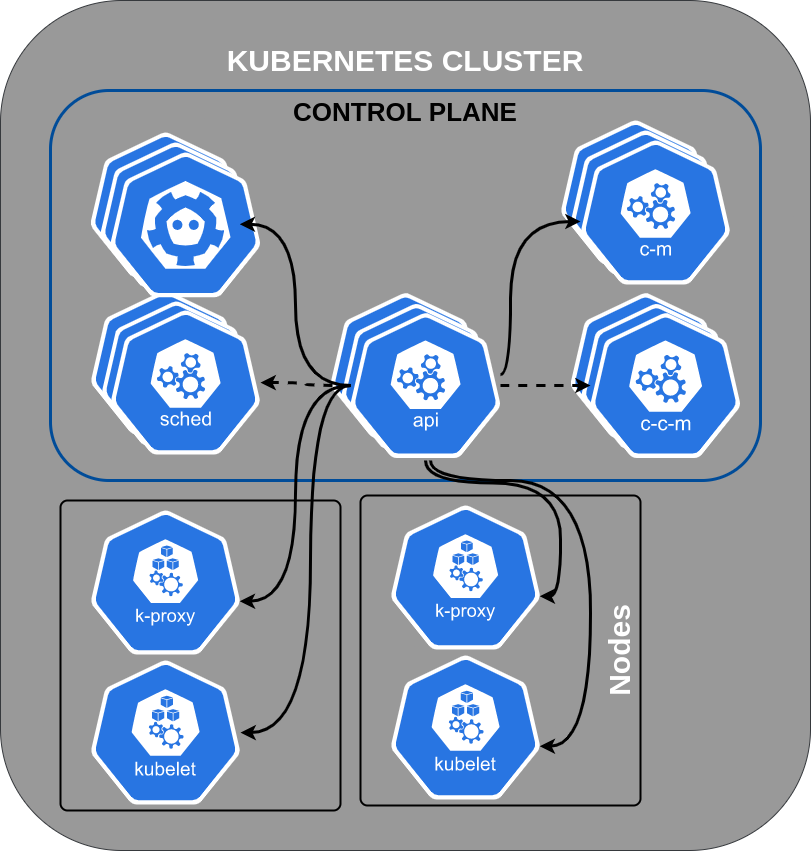
\includegraphics[width=1\textwidth]{k8s-9.png}
        \end{overprint}
        % \animategraphics[loop,autoplay,width=\linewidth]{1}{k8s-}{1}{9}
      \end{center}
    \end{column}
  \end{columns}
\end{frame}

% -- 
% Métodos
% -- 
\section{Método}

% -- 
% Abordagem
% --
\subsection{Abordagem}
\begin{frame}{Abordagem - Cluster e Análise}
  Utilizar um \emph{Cluster} Kubernetes\textregistered\ como plataforma de orquestração de cargas de trabalho em computadores desktops.
  \begin{itemize}
    \item Cargas de trabalho:
          \begin{itemize}
            \item Análise de tendência de uso de azitromicina entre 2014 e 2021
          \end{itemize}
        \item Composição do cluster com computadores \emph{desktops} reaproveitados
        \item Minimizar trabalho local e priorizar a possibilidade de provisionamneto remoto
        \item redução do CAPEX e otimizar utilização de hardware ocioso ou subutilizado
        \item reaproveitamento de maquinas
    \end{itemize}
\end{frame}

\begin{frame}{Abordagem - Condução do projeto}
  O uso de conceitos e metodologias de DevOps:
  \begin{itemize}
            \item Versionamento (Git) 
            \item CI (integração contínua) \texttt{make build}
            \item CD (entrega contínua) \texttt{make deploy}
    \item Monitoramento
        \begin{itemize}
            \item método USE, parâmetros de utilização, saturação e erro 
            \item avaliação de utilização dos nós durante processamento
        \end{itemize}
  \end{itemize}
\end{frame}

% -- 
% Especificação dos nós integrantes \emph{cluster} 
% -- 
\subsection{Especificações}

\begin{frame}[allowframebreaks]{Especificações}
      \begin{itemize}
        \item Cluster:
              \begin{itemize}
                \item Composição:
                \begin{itemize}
                    \item 1 computadores com 6 CPUs e 8GB de RAM (\emph{load balancer })
                    \item 3 computadores com 6 CPUs e 8GB de RAM (\emph{control-plane})
                    \item 4 computadores com 6 CPUs e 16GB de RAM (\emph{workers})
                \end{itemize}
              \end{itemize}
        \begin{itemize}
            \item Containers para processamento e análise:
              \begin{itemize}
                \item 90 containers (1/mês de análise) [procesamento]
                \item 1 container /  usuário [análise]
                \item arquitetura: \textbf{amd64}
                \item 1 vCPU
                \item 2 GB de RAM
              \end{itemize}
        \end{itemize}
    \end{itemize}
    
  \framebreak
  
      \begin{itemize}
        \item Orquestração do processamento dos dados originias:
              \begin{itemize}
                \item Apache Airflow\textregistered\
                \begin{itemize}
                  \item Kubernetes executor (onde)
                  \item Python Operators (como)
                \end{itemize}
              \end{itemize}
        \item Consumo e análise de dados tratados:
              \begin{itemize}
                \item JupyterHub - Notebooks para multi-usuários (gerenciamento)
                \item Jupyter Lab - Notebooks para análise dos dados (execução)
              \end{itemize}
      \end{itemize}
  
  
\end{frame}


% -- 
% Plataforma de orquestração de carga de trabalho
% -- 
\subsection{Arquitetura Orquestrador}

\begin{frame}{Arquitetura Orquestrador}
\begin{figure}
    \centering
    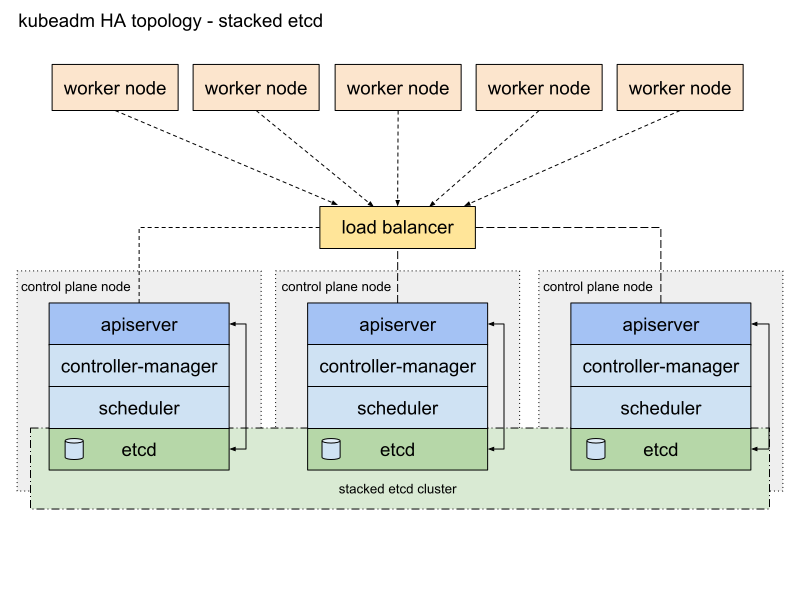
\includegraphics[width=1\textwidth]{kubeadm-ha-topology-stacked-etcd.png}
    %\caption{Caption}
    \label{fig:k8s-arch}
\end{figure}
\end{frame}

% -- 
% Configuração e provisionamento do cluster
% -- 
\subsection{Gerenciamento de configuração}

\begin{frame}{Gerenciamento de configuração}
      \begin{figure}
          \centering
      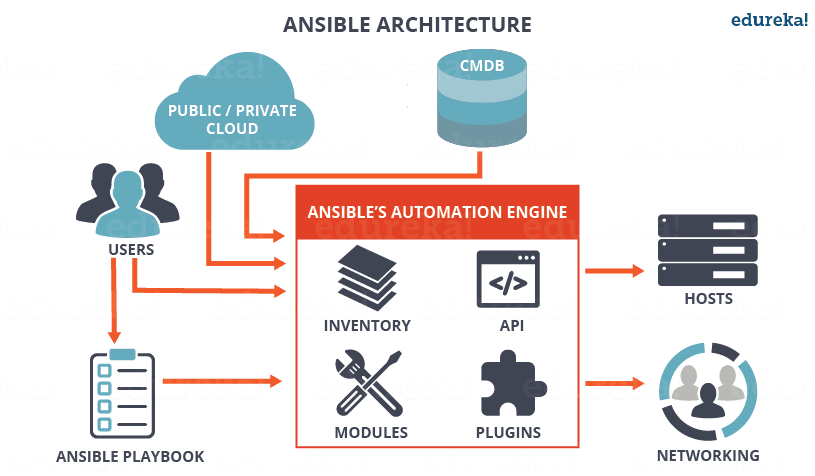
\includegraphics[width=.8\textwidth]{ansible arch.png}
          %\caption{Caption}
          \label{fig:ansiblearch}
      \end{figure}
      
\end{frame}

% -- 
% Monitoramento
% -- 
\subsection{Monitoramento}

\begin{frame}{Monitoramento}
    \begin{columns}
      \begin{column}{0.5\textwidth}
  \begin{itemize}
    \item \emph{Node Exporter} Expor métricas de Host
    \item \emph{Prometheus} -  Monitoramento de sistemas e Banco de dados de series temporais
    \item \emph{Grafana} - Dashboard e observabilidade
    \item Airflow - Relatório de tempo de execução, falhas, tentativas
  \end{itemize}
\end{column}
\begin{column}{0.5\textwidth}
  \begin{center}
    \begin{figure}
      \centering
      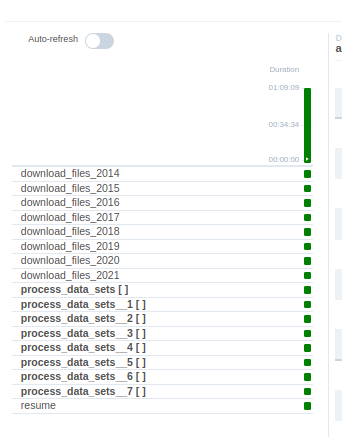
\includegraphics[width=.9\textwidth]{report_execution_summary.png}
      \caption{Airflow - Relatório de execução}
    \end{figure}
  \end{center}
\end{column}
\end{columns}
\end{frame}


% -- 
% Comparação entre tipos de virtualização
% -- 
\subsection{Avaliação viabilidade}

\begin{frame}[allowframebreaks]{Avaliação de utilização do cluster}
  
  \begin{itemize}
      \item macrobenchmark (system level benchmark) - Teste utizando uma solução avaliando tempo de execução
      \item[] métricas de Desempenho (nós do cluster, \emph{guests}):
      \item Taxa de Utilização de CPU e Memória 
      \item Taxa de saturação de CPU e Memória
      \item[] Tempo de Implementação:
      \item Tempo de configuração do cluster
      \item[] Método base utilizado para coleta de informações:
      \item Metodo USE de avaliação (Checklist Linux)
  \end{itemize}
\end{frame}


% -- 
% Análise de dados
% -- 
\subsection{Análise de dados}

\begin{frame}{Exemplo da Análise de dados}
  \begin{itemize}
    \item Vendas de Medicamentos Controlados e Antimicrobianos - Medicamentos Industrializados
    \item $530 \cdot 10^{6}$ linhas com mais de 70 GB
    \item Análise de tendência do consumo de azitromicina por região
    \item Análise de tendência do consumo de azitromicina no país
    \item Avaliação compartiva de 2 anos anteriores ao COVID-19
  \end{itemize}
\end{frame}

% -- 
% Cronograma
% -- 
% \subsection{Cronograma}

% \begin{frame}[plain]
%   \hspace*{-10mm}
%   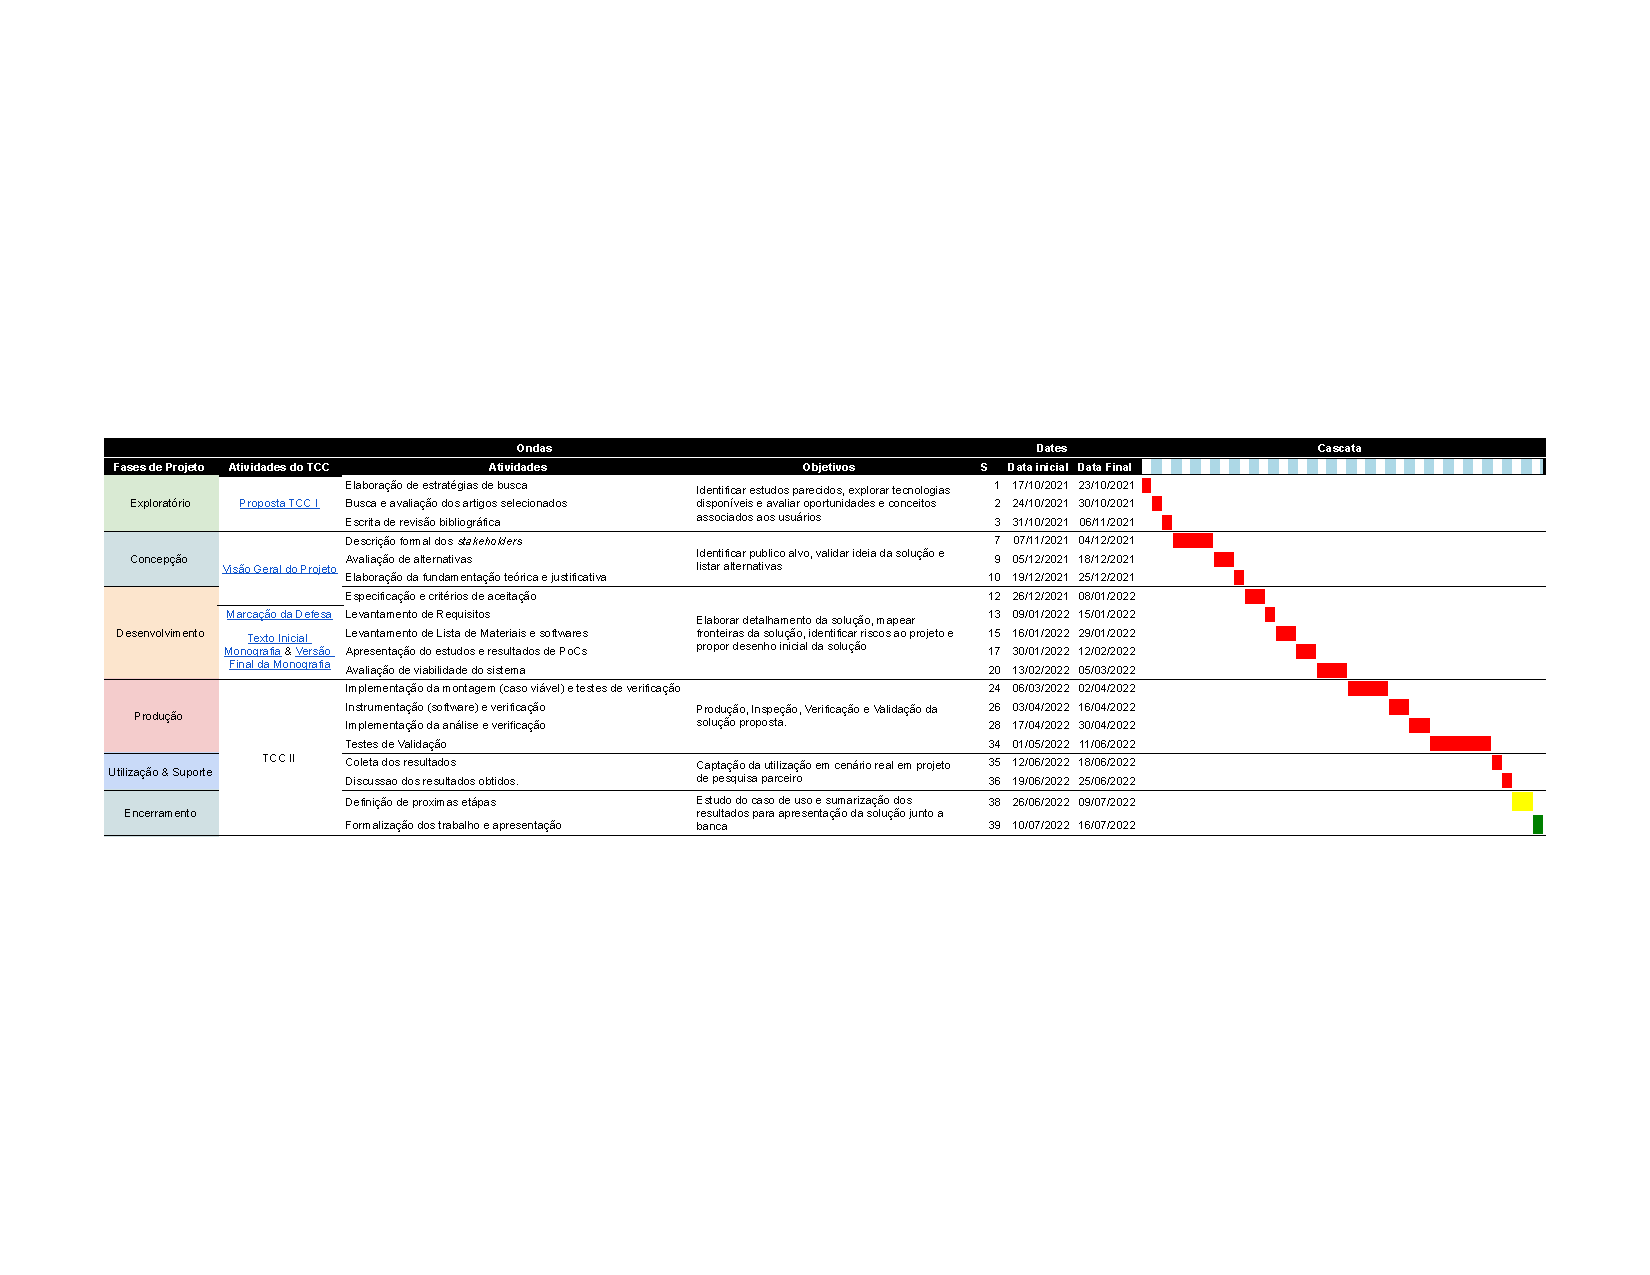
\includegraphics[width=\paperwidth]{TCC cronograma - Sheet1.pdf}
% \end{frame}


% -- 
% Disponibilidade dos recursos deste trabalho
% -- 
\section{Resultados}

\begin{frame}{Disponibilidade dos recursos}
  Todos os componentes definidos neste trabalho estarão contidos em um repositório público \href{https://github.com/felipefrocha/esufmg-tcc}{https://github.com/felipefrocha/esufmg-tcc}, sob a licença pública geral GNU versão 3, para livre acesso.
\end{frame}

\subsection{Provisionamento}

\begin{frame}
  \hspace*{-15mm}
  \begin{figure}
      \centering
      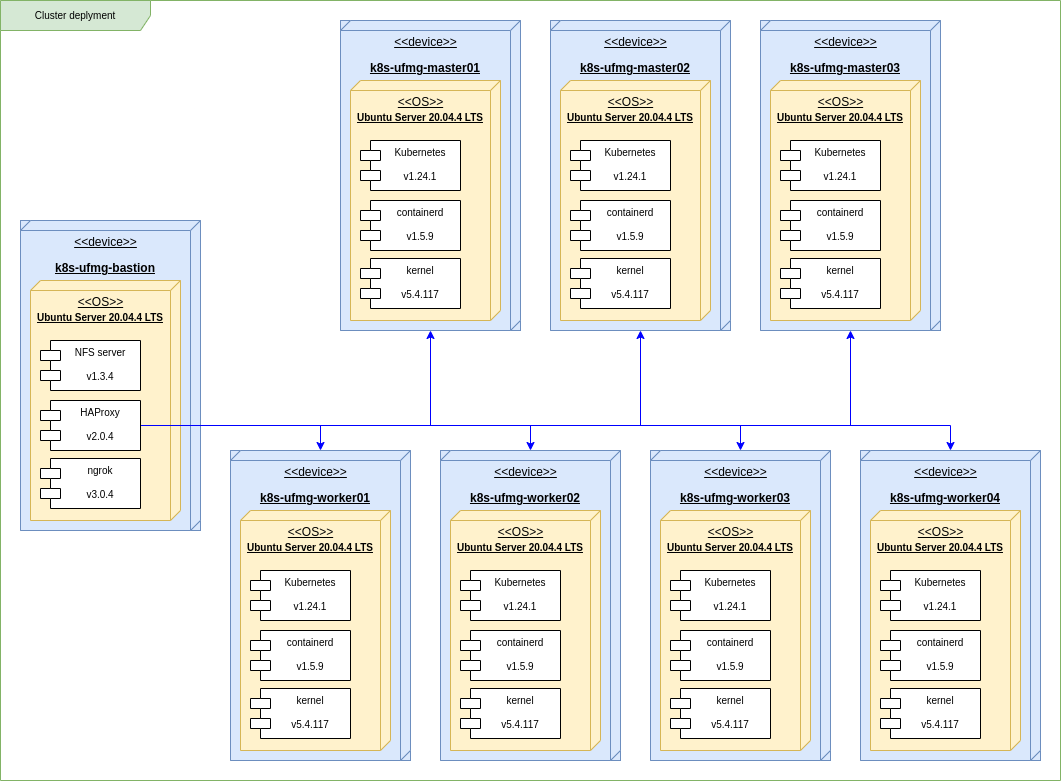
\includegraphics[width=.9\textwidth]{TCC - Kubenertes-Cluster Deplyment.drawio.png}
      \caption{Diagrama de deploy - OS e versões}
      \label{fig:k8s-arch-deploy}
  \end{figure}
  \end{frame}

\begin{frame}[plain]{NgRok - Acesso Remoto}
  \hspace*{-10mm}
  \begin{figure}
    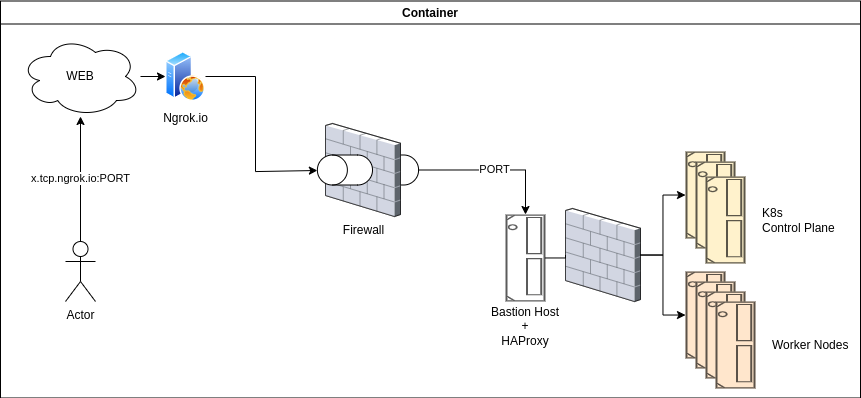
\includegraphics[width=.85\paperwidth]{ngroktcp.png}
  \caption[Funcionamnto NgRok]{Funcionamento NgRok}
  \end{figure}
\end{frame}

\begin{frame}[plain]{NgRok - Painel}
 \hspace*{-10mm}
  \begin{figure}
    \centering  
  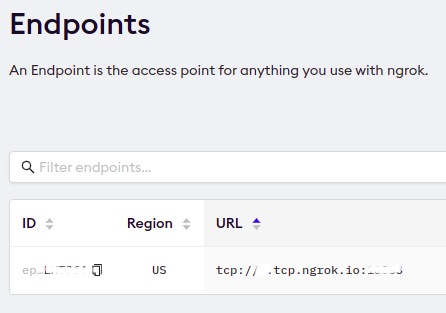
\includegraphics[width=0.5\paperwidth]{ngrok.png}
\end{figure}
\end{frame}


% \begin{frame}[plain]
%   \hspace*{-10mm}
%   \begin{figure}
%     \centering  
%     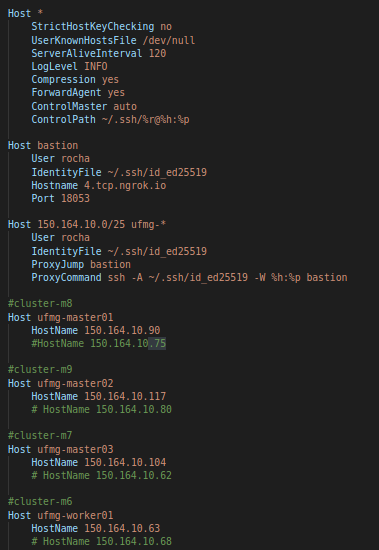
\includegraphics[height=0.6\paperwidth]{ssh.png}
%     \caption[ssh config]{SSH config}
%   \end{figure}
% \end{frame}

% \begin{frame}[plain]
%   \hspace*{-10mm}
%   \begin{figure}
%     \centering  
%     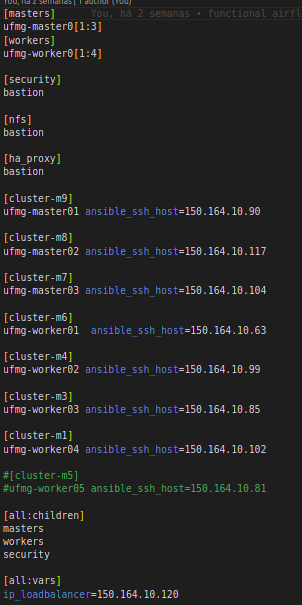
\includegraphics[height=0.6\paperwidth]{ansible_inventory.png}
%     \caption[Ansible inventory]{Ansible inventory}
%   \end{figure}
% \end{frame}
\subsection{Configuração}

\begin{frame}[plain]
  \hspace*{-10mm}
    \begin{figure}
      \begin{center}
        % 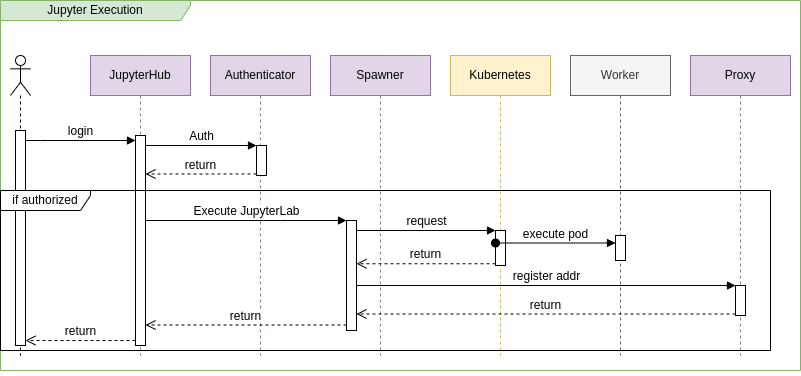
\includegraphics[width=.85\paperwidth]{jupyter_sequence.png}
        \begin{overprint}
          \onslide<1>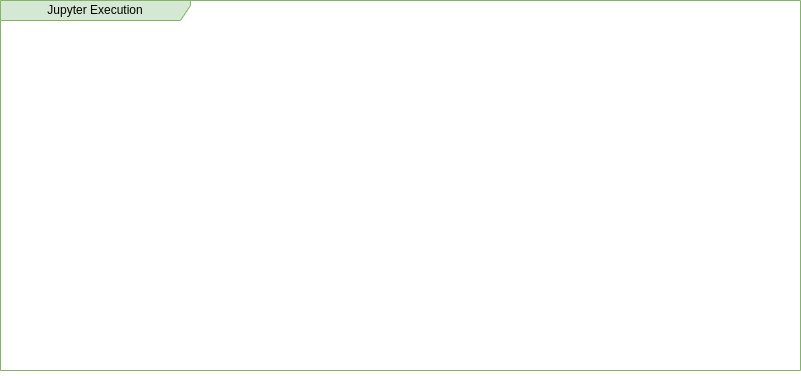
\includegraphics[width=1\textwidth]{seq-jupy-1.png}
          \onslide<2>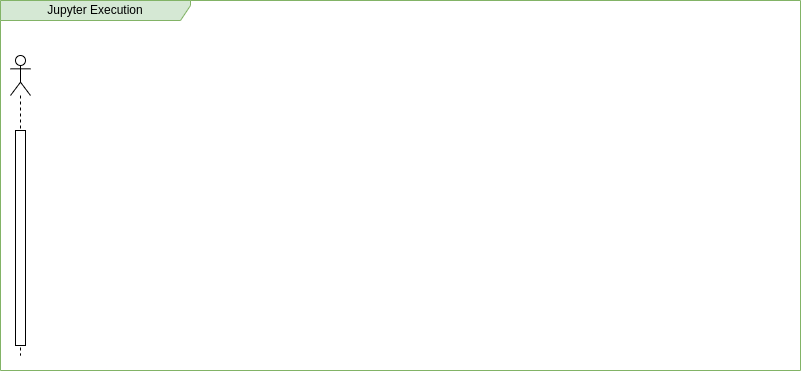
\includegraphics[width=1\textwidth]{seq-jupy-2.png}
          \onslide<3>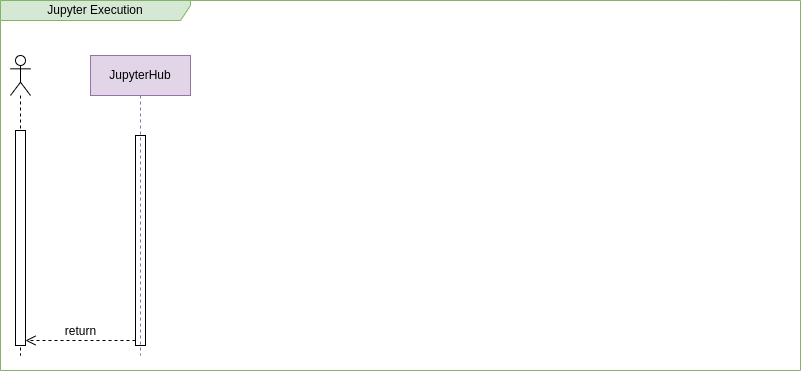
\includegraphics[width=1\textwidth]{seq-jupy-3.png}
          \onslide<4>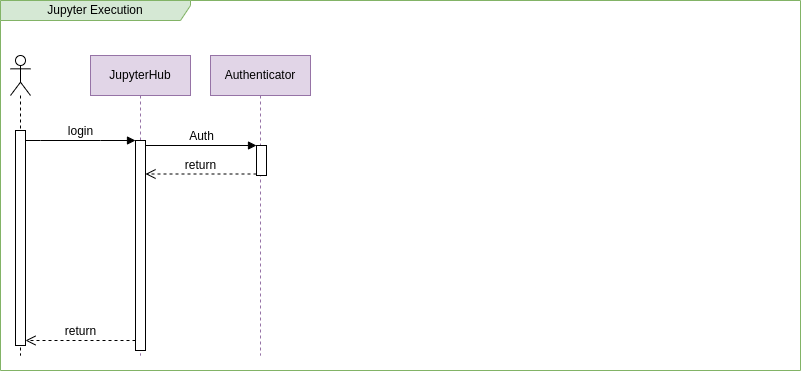
\includegraphics[width=1\textwidth]{seq-jupy-4.png}
          \onslide<5>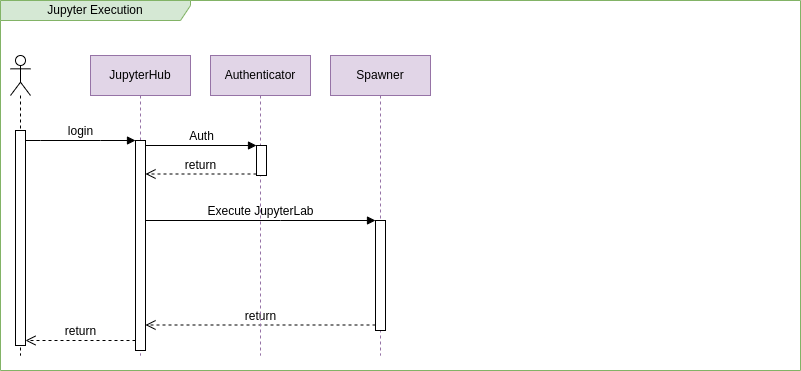
\includegraphics[width=1\textwidth]{seq-jupy-5.png}
          \onslide<6>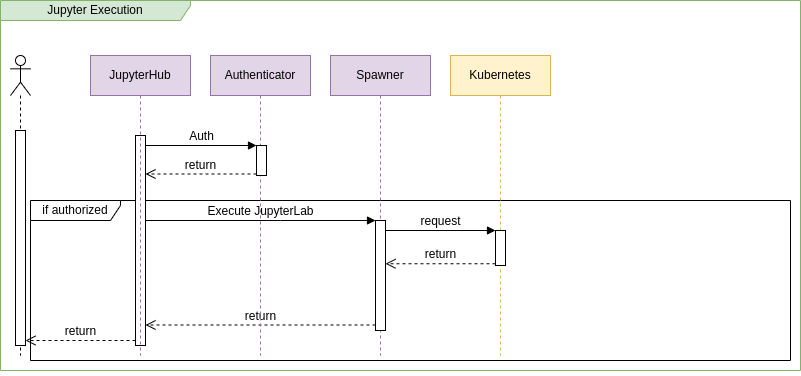
\includegraphics[width=1\textwidth]{seq-jupy-6.png}
          \onslide<7>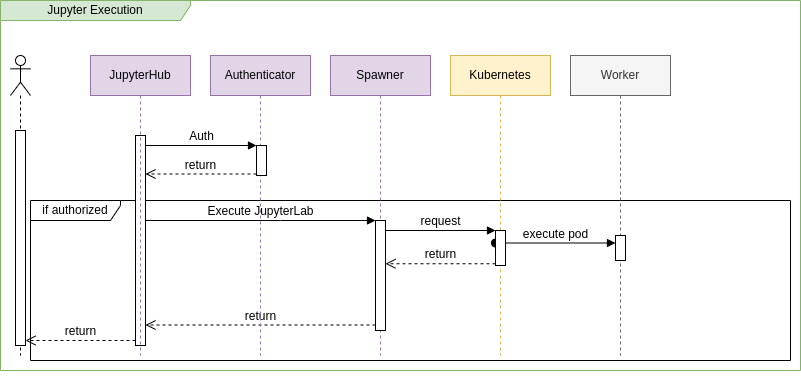
\includegraphics[width=1\textwidth]{seq-jupy-7.png}
          \onslide<8->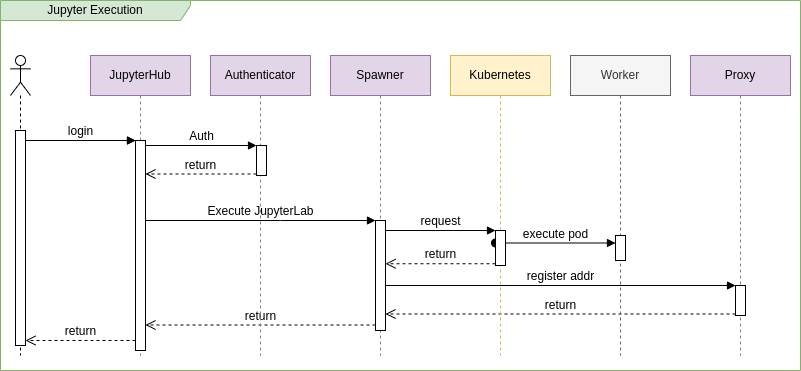
\includegraphics[width=1\textwidth]{seq-jupy-8.png}
        \end{overprint}
      \end{center}  
      \caption[Jupyter - Diagrama de Sequencia]{Jupyter - Diagrama de Sequencia}
  \end{figure}  
\end{frame}

\begin{frame}[plain]
  \hspace*{-10mm}
  \begin{figure}
  % 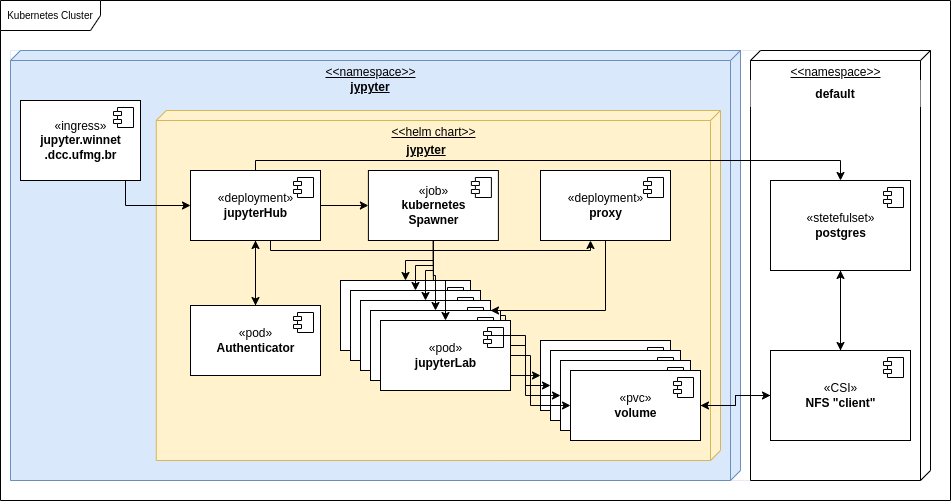
\includegraphics[width=0.85\paperwidth]{tcc_jupyter_deploy.png}
  \begin{center}
    % 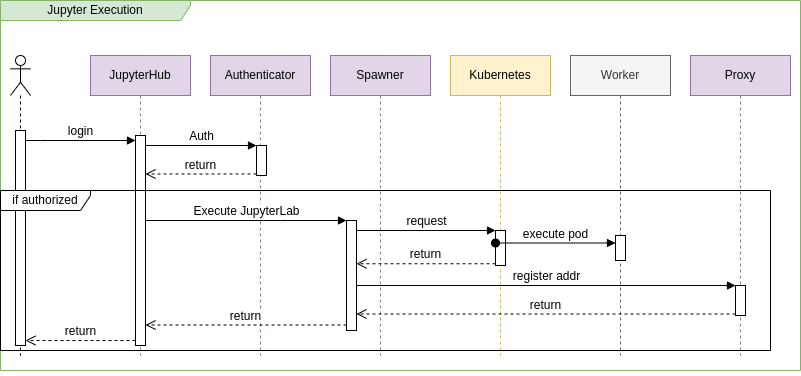
\includegraphics[width=.85\paperwidth]{jupyter_sequence.png}
    \begin{overprint}
      \onslide<1>
\includegraphics[width=1\textwidth]{deploy-jupy-1.png}
      \onslide<2>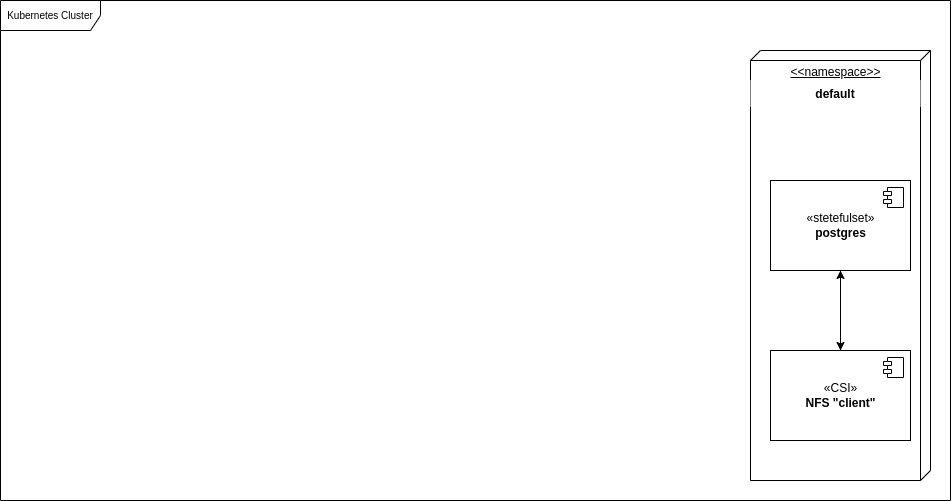
\includegraphics[width=1\textwidth]{deploy-jupy-2.png}
      \onslide<3>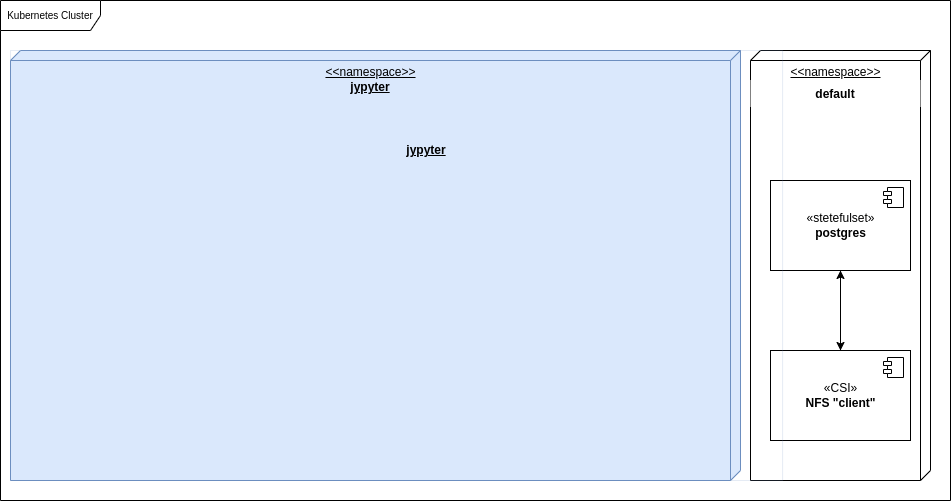
\includegraphics[width=1\textwidth]{deploy-jupy-3.png}
      \onslide<4>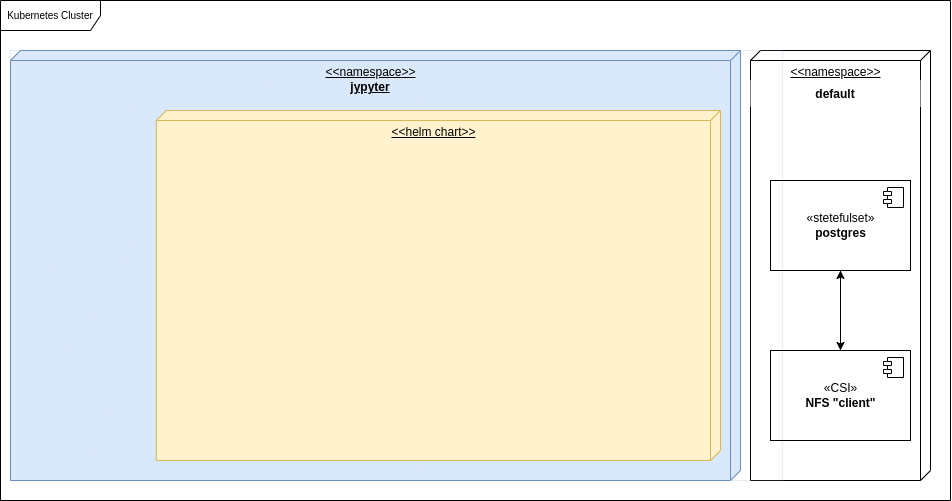
\includegraphics[width=1\textwidth]{deploy-jupy-4.png}
      \onslide<5>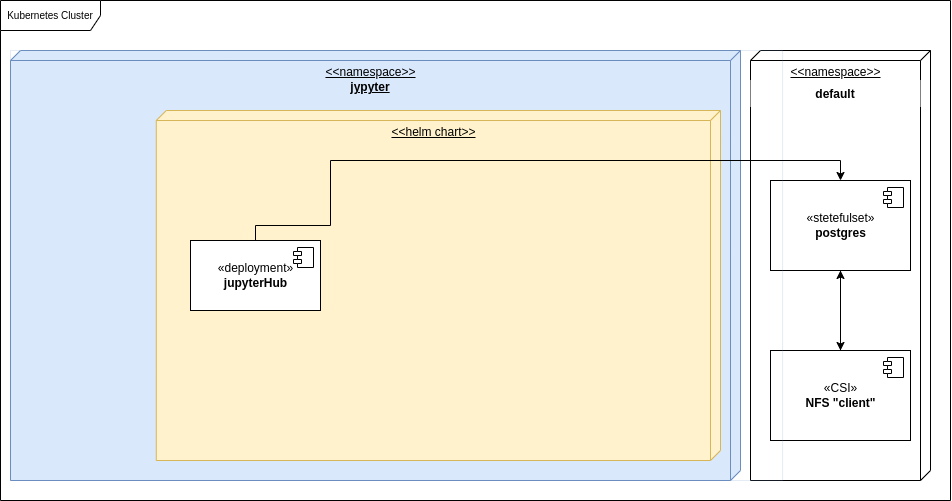
\includegraphics[width=1\textwidth]{deploy-jupy-5.png}
      \onslide<6>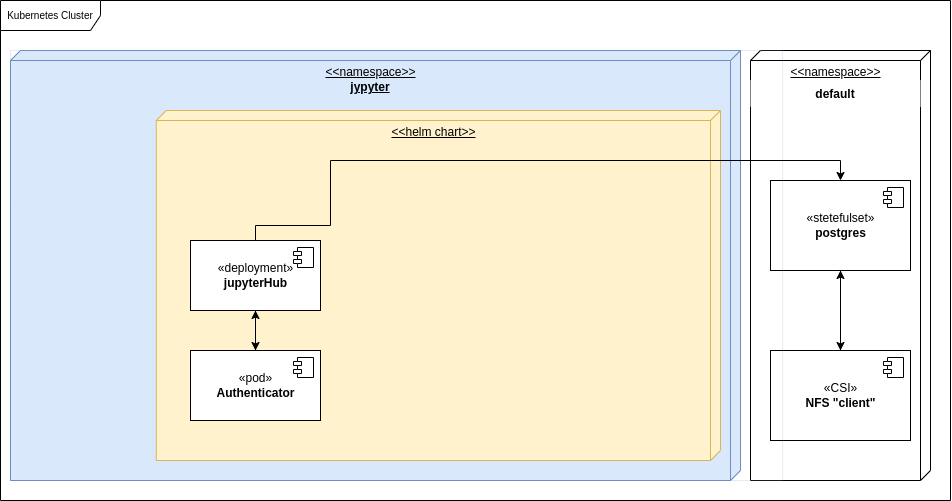
\includegraphics[width=1\textwidth]{deploy-jupy-6.png}
      \onslide<7>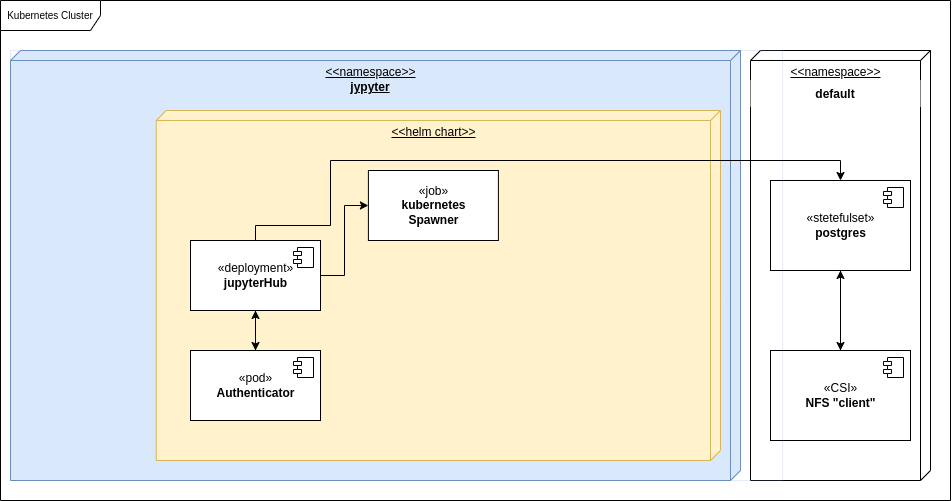
\includegraphics[width=1\textwidth]{deploy-jupy-7.png}
      \onslide<8>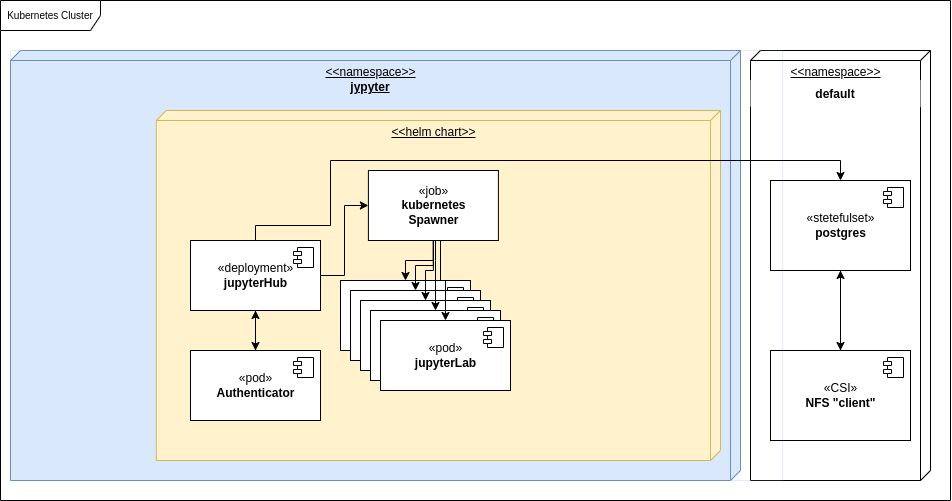
\includegraphics[width=1\textwidth]{deploy-jupy-8.png}
      \onslide<9>\includegraphics[width=1\textwidth]{deploy-jupy-9.png}
      \onslide<10>\includegraphics[width=1\textwidth]{deploy-jupy-10.png}
      \onslide<11>\includegraphics[width=1\textwidth]{deploy-jupy-11.png}
      \onslide<12->\includegraphics[width=1\textwidth]{deploy-jupy-12.png}
    \end{overprint}
  \end{center}  
      \caption[Jupyter Deploy]{Jupyter - Diagrama de Deploy}
  \end{figure}  
\end{frame}

\begin{frame}[plain]
  \hspace*{-10mm}
    \begin{figure}
    \centering  
  \includegraphics[width=.85\paperwidth]{airflow_sequence.png}
      \caption[Airflow - Diagrama de Sequencia]{Airflow - Diagrama de Sequencia}
  \end{figure}  
\end{frame}

\begin{frame}[plain]
  \hspace*{-10mm}
  \begin{figure}
    \centering  
  \includegraphics[width=0.85\paperwidth]{tcc_airflow_deloy.png}
  \caption[AirFlow Deploy]{Ariflow - Diagrama de Deploy}
\end{figure}
\end{frame}

\begin{frame}[plain]
  \hspace*{-10mm}
  \begin{figure}
    \centering  
  \includegraphics[width=.85\paperwidth]{tcc_monitoring_deploy.png}
      \caption[Monitoramento deploy]{Monitoramento - Diagrama de Deploy}
  \end{figure}  
\end{frame}

\begin{frame}[plain]
  \hspace*{-10mm}
  \begin{figure}
    \centering  
  \includegraphics[width=.85\paperwidth]{fluxo_processo.png}
      \caption{Fluxo de Process - Diagrama de Fluxo}
  \end{figure}  
\end{frame}

\begin{frame}[plain]
  \hspace*{-10mm}
  \begin{figure}
    \begin{center}
      % \includegraphics[width=.85\paperwidth]{jupyter_sequence.png}
      \begin{overprint}
        \onslide<1>\includegraphics[width=1\textwidth]{flow-1.png}
        \onslide<2>\includegraphics[width=1\textwidth]{flow-2.png}
        \onslide<3>\includegraphics[width=1\textwidth]{flow-3.png}
        \onslide<4>\includegraphics[width=1\textwidth]{flow-4.png}
        \onslide<5>\includegraphics[width=1\textwidth]{flow-5.png}
        \onslide<6>\includegraphics[width=1\textwidth]{flow-6.png}
        \onslide<7->\includegraphics[width=1\textwidth]{flow-7.png}
      \end{overprint}
    \end{center}  
      \caption{Processo ETL - Diagrama de Fluxo}
  \end{figure}  
\end{frame}

\begin{frame}{Resultados e discussões}
  \begin{itemize}
    \item Provisionamento
    \begin{itemize}
      \item Tempo de configuração inicial
      \begin{itemize}
        \item cloud-init: 2h (possivel redução  se utilizado imagens em rede)
      \end{itemize}
    \end{itemize}
    \begin{itemize}
      \item Tempo de configuração cluster
        \begin{itemize}
          \item automação de configuração Ansible: $20-35m$
          \item Helm (deploy aplicação) + Terraform (orquestração de deploy): $10-25m$
        \end{itemize}
    \end{itemize}
    \item execução dos job ($2GB$ de RAM e $1CPU$, $90$ pods):
    \begin{itemize}
        \item Tempo ingestão dos dados: $\approx 53m$ 
    \end{itemize}
    % \item Lead Time:
    % \begin{itemize}
    %     \item Tempo de deploy Airflow DAG: $3-6m$
    %     \item Tempo de deploy JupyterLab: $4-10m$
    % \end{itemize}
  \end{itemize}
\end{frame}


\begin{frame}[plain]
  \hspace*{-10mm}
  \begin{figure}
    \centering  
  \includegraphics[width=.75\paperwidth]{s3_size.png}
      \caption{S3 Lista de arquivos}
  \end{figure}  
\end{frame}

\begin{frame}[plain]
  \hspace*{-10mm}
  \begin{figure}
    \centering  
  \includegraphics[width=.5\paperwidth]{report_execution_summary.png}
      \caption[Airflow relatório]{Relatório de orquestração}
  \end{figure}  
\end{frame}

\begin{frame}[plain]
  \hspace*{-10mm}
  \begin{figure}
    \centering  
  \includegraphics[width=.75\paperwidth]{graph_execution.png}
      \caption[Airflow relatório]{grafo DAG}
  \end{figure}  
\end{frame}


\subsection{Resultados do Monitoramento}

\begin{frame}[plain]
  \hspace*{-10mm}
  \begin{figure}
    \centering  
  \includegraphics[width=.5\paperwidth]{report_execution_summary1.png}
      \caption[Airflow relatório]{Relatório de Orquestração}
  \end{figure}  
\end{frame}

\begin{frame}[plain]
  \hspace*{-10mm}
  \begin{figure}
    \centering  
  \includegraphics[width=.75\paperwidth]{etl_1_usage.png}
      \caption[Monitoramento execução]{Monitoramento execução}
  \end{figure}  
\end{frame}

% \begin{frame}[plain]
%   \hspace*{-10mm}
%     \begin{figure}
%     \centering  
%   \includegraphics[width=.75\paperwidth]{etl_2_usage.png}
%       \caption[Monitoramento execução 2]{Monitoramento execução 2}
%   \end{figure}  
% \end{frame}

% \begin{frame}[plain]
%   \hspace*{-10mm}
%     \begin{figure}
%     \centering  
%   \includegraphics[width=.75\paperwidth]{etl_3_usage.png}
%       \caption[Monitoramento execução 3]{Monitoramento execução 3}
%   \end{figure}  
% \end{frame}

\begin{frame}[plain]
  \hspace*{-10mm}
    \begin{figure}
    \centering  
  \includegraphics[width=.6\paperwidth]{jupyter_consumption.png}
      \caption[Monitoramento Jupyter]{Monitoramento Jupyter}
  \end{figure}  
\end{frame}

\begin{frame}[plain]
  \hspace*{-10mm}
    \begin{figure}
    \centering  
  \includegraphics[width=.6\paperwidth]{postgres_resource.png}
      \caption[Monitoramento Postgres]{Monitoramento Postgres}
  \end{figure}  
\end{frame}

\subsection{Resultados das Análises}
\begin{frame}{Resultados das Análises}

    \begin{itemize}
      \item Total de prescrições 95.345.640 
      % \item População:
      % \begin{itemize}
      %   \item Maioria sexo femnino: $53,62\%$
      %   \item Idade: $\bar{x} = 32,75 \pm 2,04$
      % \end{itemize}
      \item Aumento de prescrições de $+32,1\%$ (2014-2020)
      \item Prescrições por $1000 hab$: $+26,59\%$ (2014-2020)
      
      \item Regiões:
        \begin{itemize}
          \item Sudeste: $47,44\%$ $\{MG: 13,17,SP: 24,76\%\}$
          \item Sul: $22,47\%$ $\{RS: 12,49\%\}$
        \end{itemize}
      \item Estados destaque para aumento:  Minas Gerais ($+125,38\%$), Rondônia ($+191,73\%$ e Roraima ($+168,27\%$))
    \end{itemize}
\end{frame}


% \begin{frame}[plain]
%   \hspace*{-10mm}
%     \begin{figure}
%     \centering  
%   \includegraphics[width=.6\paperwidth]{distribuicao_sexo.png}
%       \caption{Pescrição por sexo por UF}
%   \end{figure}  
% \end{frame}

\begin{frame}[plain]
  \hspace*{-10mm}
    \begin{figure}
    \centering  
  \includegraphics[width=.6\paperwidth]{distribuicao_presc_ano.png}
      \caption{Presciçõe por ano}
  \end{figure}  
\end{frame}


\begin{frame}[plain]
  \hspace*{-10mm}
    \begin{figure}
    \centering  
  \includegraphics[width=.6\paperwidth]{distribuicao_presc_ano_estado.png}
      \caption{Prescições por por ano por UF}
  \end{figure}  
\end{frame}

    \begin{frame}{Resultados das Análises}


  Relevância estatística ($p$ valor) para correlação por $\tau$ de Kendall:
    \begin{table}[]
      \begin{tabular}{ccc}
      \hline
      \multicolumn{1}{c}{\textbf{UF}} & \multicolumn{1}{c}{\textbf{$\tau$}} & \multicolumn{1}{c}{\textbf{$p$ valor}} \\ \hline
      MT                              & 1.0                         & 0.003                            \\
      RJ                              & 1.0                         & 0.003                            \\
      RN                              & 1.0                         & 0.003                            \\
      RO                              & 1.0                         & 0.003                            \\
      TO                              & 0.87                         & 0.017                            \\ \hline
      \end{tabular}
      \end{table}
\end{frame}

% -- 
% Conclusão
% -- 
\section{Conclusão}

\begin{frame}{Conclusão}
  \begin{itemize}
    \item Entendimento da complexidade dos fatores considerados no processo de decisão em saúde
    \item Análise dos impactos sociais-econômicos relativos a restrição orçamentária na ciência
    \item Seleção de tecnologias com base em requisitos e restrições
    \item Stack de tecnologia de mercado (maior suporte e melhores praáticas)
    \item Desenho de uma estratégia de extração de informações em saúde
    \item Avaliação da viabilidade de uso de clusters de baixo custo na processamento de dados
    \item Interdisciplinariedade, especificidade e especialidade
    \item Produção de conhecimento de suporte prático 
    \item Viés politico nas descisões em saúde. 
    \item Observabilidade dos dados em saúde
  \end{itemize}
\end{frame}
\begin{frame}{Conclusão}
  
  Para trabalho futuro visa se a otimizaçao de estratégia de dimensionamento de recursos, avaliação comparativa de outras técnologias e técnicas para abordar o problema de processamneto paralelo e distribuído.
  Ainda sugere-se, baseado nos resultados desse trabalho, discutir formas de recrutamento de computadores para o \emph{cluster} de outros laboratórios, de maneira a criar elasticidade para cargas de trabalho ainda mais extensas.
\end{frame}


% -- 
% Referências
% -- 
\begin{frame}[allowframebreaks]{Referências}
  \small
  %	\nocite{*}
  %    \bibliographystyle{apalike}
  \bibliography{Apresentacao}
\end{frame}


\begin{frame}
  \centering
  {\color{ros} OBRIGADO\\
    :)}
\end{frame}
\end{document}